\documentclass[a4paper, 12pt]{article}
\usepackage[utf8]{inputenc}
\usepackage[english,russian]{babel}
\usepackage[warn]{mathtext}
\usepackage{graphicx}
\usepackage{float}
\restylefloat{table}
\usepackage{amsmath}
\usepackage{floatflt}
\usepackage[T2A]{fontenc}
\usepackage[left=20mm, top=20mm, right=20mm, bottom=20mm, footskip=10mm]{geometry}

\tolerance 1414
\hbadness 1414
\emergencystretch 1.5em
\hfuzz 0.3pt        % размер максимального переполнения без warning'a
\widowpenalty=10000 % запрещает одиночную строку абзаца в начале страницы
\vfuzz \hfuzz
\raggedbottom       % если на странице мало содержимого, добавить пустое место в конце, а не в середине страницы



\begin{document}

\begin{titlepage}
	\centering
	\vspace{5cm}
	{\scshape\LARGE московский физико-технический институт (национальный исследовательский университет) \par}
	\vspace{6cm}
	{\scshape\Large Лабораторная работа 3.3.1 \par}
	{\huge\bfseries Изучение удельного заряда электрона \par}
	\vspace{1cm}
	\vfill
\begin{flushright}
	{\large Б03-102}\par
	\vspace{0.3cm}
	{\LARGE Куланов Александр}
\end{flushright}
	

	\vfill


	Долгопрудный, 2022 г.
\end{titlepage}

\section{Метод магнитной фокусировки}

\begin{itemize}
	\item \textbf{Цель работы:} Определение значения магнитных полей, при которых происходит фокусировка электронного пучка, и по результатам измерений считать удельный заряд электрона $e/m$.
    \item \textbf{В работе используются:} Электронно-лучевая трубка и блок питания к ней; источник постоянного тока; соленоид; электростатический вольтметр; милливеберметр; ключи.
\end{itemize}

\subsection{Описание установки}
\begin{figure}[H]
    \centering
    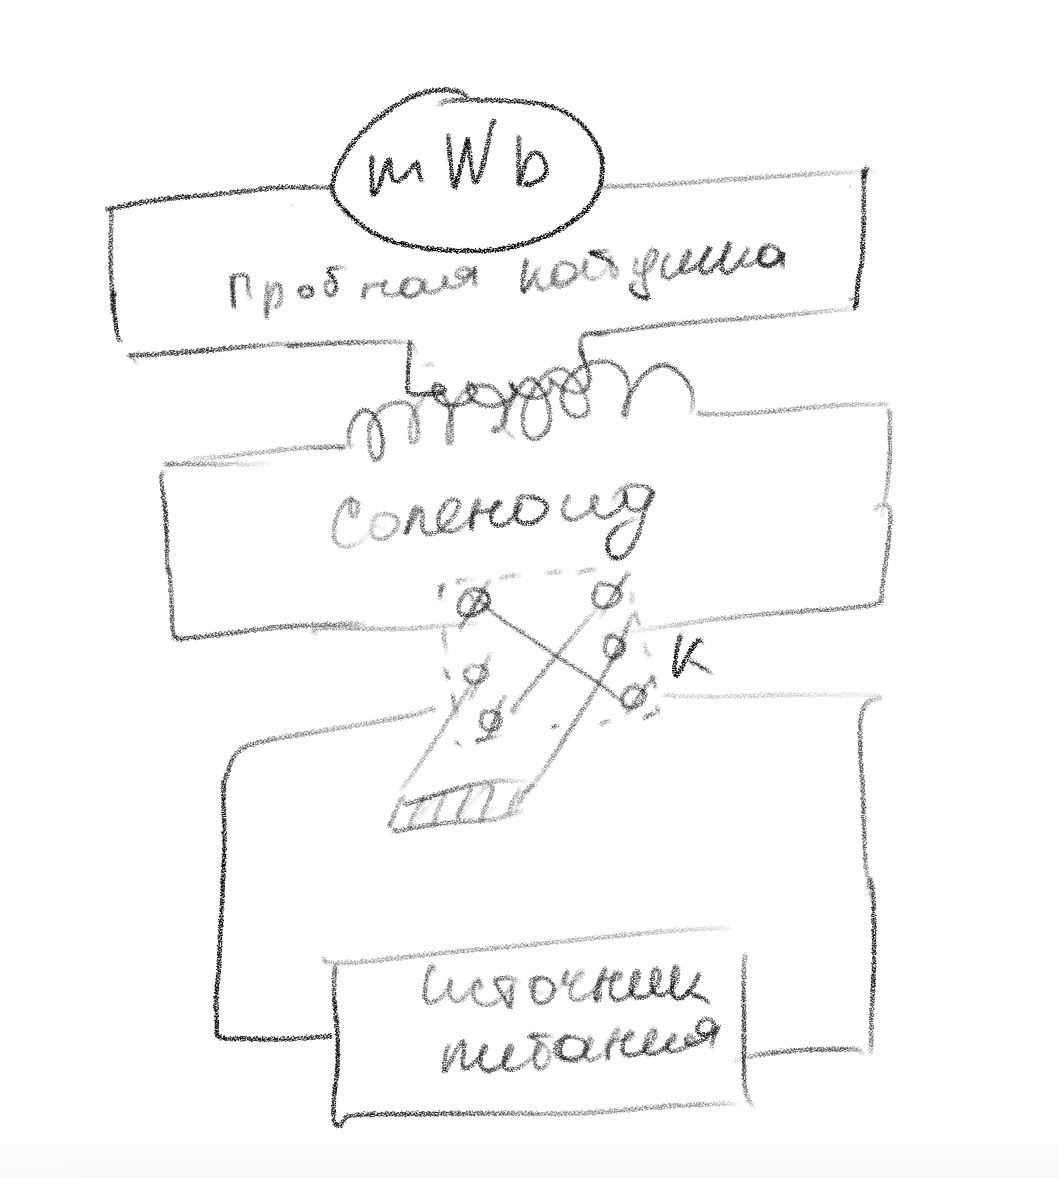
\includegraphics[width=0.7\textwidth]{set}
    \caption{Схема установки}
    \label{fig:set}
\end{figure}
Основной частью установки является электронный осциллограф, трубка которого вынута и установлена в длинном соленоиде, создающим магнитное поле. Напряжение на отклоняющие пластины и питание подводятся к трубке многожильным кабелем.

Пучок электронов, вылетающих из катода с разными скоростями, ускоряется анодным напряжением. Пропустив пучок сквозь две узкие диафрагмы, можно выделить электроны с практически одинаковой продольной скоростью. Небольшое переменное напряжение, поступающее с клеммы "Контрольный сигнал" осциллографа на отклоняющие пластины, изменяет только поперечную составляющую скорости. При увеличении магнитного поля линия на экране стягивается в точку, а затем снова удлиняется. 

Магнитное поле создается постоянным током, величина которого регулируется ручками источника питания и измеряется амперметром. Ключ служит для изменения направления поля в соленоиде.

Величина магнитного поля определяется с помощью милливеберметра.

На точность результатов может влиять внешнее магнитное поле, особенно продольное. 

Измерения магнитного поля с помощью милливеберметра обычно проводятся в предварительных опыта: при отключении ключа устанавливается связь между силой тока и индукцией магнитного поля в соленоиде. 

\subsection{Теоретические сведения}
При калибровке учитываем, что 
\begin{equation}
	\Phi = BSN \Rightarrow B = \frac{\Phi}{SN}
\end{equation}
Далее, имеем
\begin{equation}
	B = kn \Rightarrow \frac{n}{B(n)} = \frac{1}{k}
\end{equation}
где k получено при аппроксимации данных для фокусировки. Удельный заряд электрона тогда
\begin{equation}
\dfrac{e}{m_e} = \dfrac{8\pi^2V}{l^2} \dfrac{n^2}{B^2(n)} = \dfrac{8\pi^2V}{l^2} \dfrac{1}{k^2},
\label{eq:main}
\end{equation}
где $V$ - ускоряющий потенциал в электронной трубке, $l$ - путь электрона, $B(n)$ - фокусирующее поле, $n$ - номер фокуса.

\subsection{Обработка результатов}
Приведем сведения об установке:
\begin{table}[H]
	\centering
	\begin{tabular}{|c|c|}
	\hline
	Величина & Значение \\ \hline
	l, \text{м}     & 0,265    \\ \hline
	SN, $\text{м}^2$  & 0,3      \\ \hline
	$V$, \text{кВ} & 0,8	\\ \hline
	\end{tabular}
	\caption{Данные установки}
	\label{tab:data}
\end{table}
Данные, полученные во время опыта занесем в таблицу:
\begin{table}[H]
	\centering
	\begin{tabular}{|ccc|ccc|}
	\hline
	\multicolumn{3}{|c|}{Прямое направление}                              & \multicolumn{3}{c|}{Обратное направление}                            \\ \hline
	\multicolumn{1}{|c|}{I, A} & \multicolumn{1}{c|}{Ф, мВб/дел} & В, мТл & \multicolumn{1}{c|}{I, A} & \multicolumn{1}{c|}{Ф, мВб/дел} & В, мТл \\ \hline
	\multicolumn{1}{|c|}{0,57} & \multicolumn{1}{c|}{0,7}        & 2,3    & \multicolumn{1}{c|}{0,59} & \multicolumn{1}{c|}{-0,9}       & 3      \\ \hline
	\multicolumn{1}{|c|}{1,15} & \multicolumn{1}{c|}{1,4}        & 4,7    & \multicolumn{1}{c|}{1,16} & \multicolumn{1}{c|}{-1,6}       & 5,3    \\ \hline
	\multicolumn{1}{|c|}{1,72} & \multicolumn{1}{c|}{2,1}        & 7      & \multicolumn{1}{c|}{1,73} & \multicolumn{1}{c|}{-2,4}       & 8      \\ \hline
	\multicolumn{1}{|c|}{2,31} & \multicolumn{1}{c|}{3}          & 10     & \multicolumn{1}{c|}{2,31} & \multicolumn{1}{c|}{-3,3}       & 11     \\ \hline
	\multicolumn{1}{|c|}{2,89} & \multicolumn{1}{c|}{3,8}        & 12,7   & \multicolumn{1}{c|}{2,88} & \multicolumn{1}{c|}{-4}         & 13,3   \\ \hline
	\multicolumn{1}{|c|}{3,45} & \multicolumn{1}{c|}{4,5}        & 15     & \multicolumn{1}{c|}{3,46} & \multicolumn{1}{c|}{-4,7}       & 15,7   \\ \hline
	\end{tabular}
	\caption{Калибровочные данные}
	\label{tab:data_1}
\end{table}
По калибровочным данным найдем, как B зависит от I:
\begin{figure}[H]
    \centering
    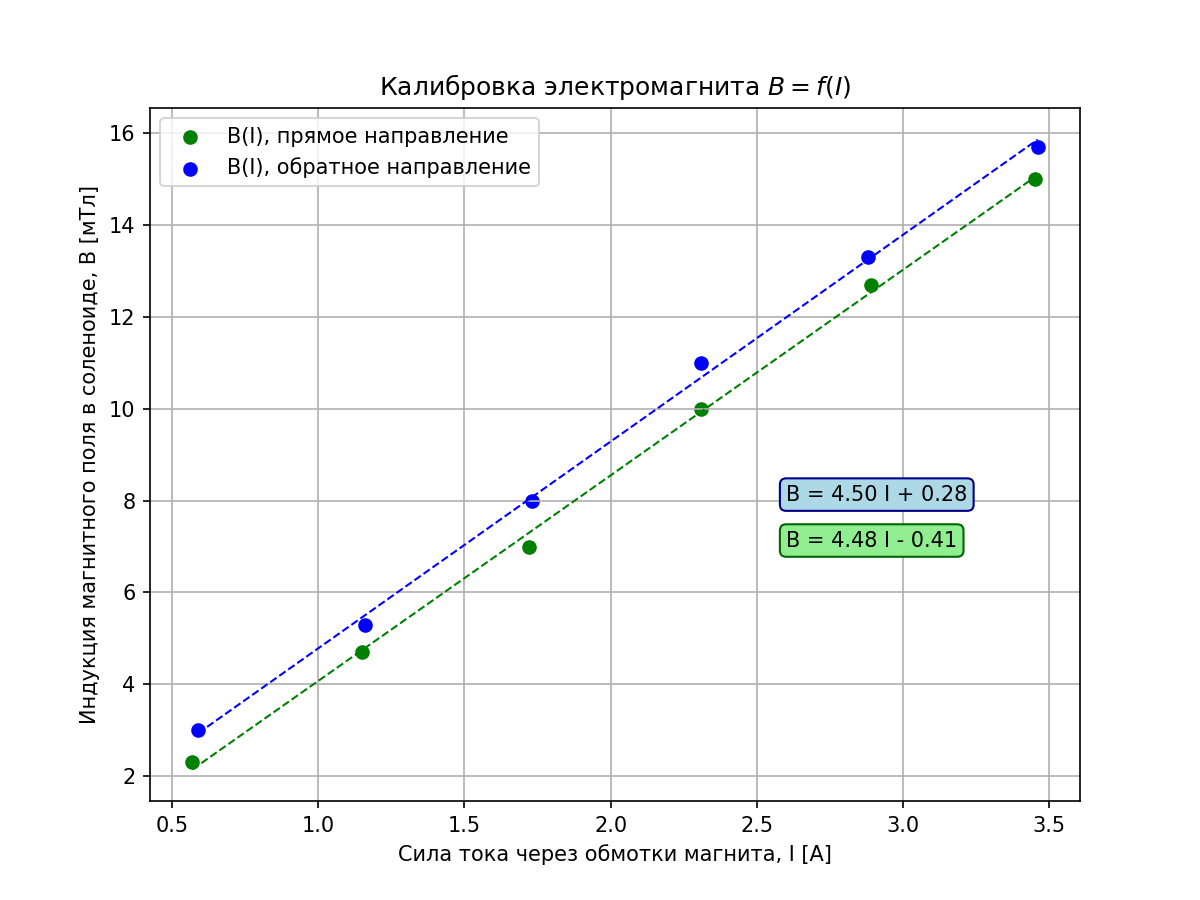
\includegraphics[width=1\textwidth]{calib.png}
    \caption{Калибровка}
    \label{fig:calib}
\end{figure}
Далее занесем в таблицу данные по определнию фокусирующего тока:
\begin{table}[H]
	\centering
	\begin{tabular}{|ccc|ccc|}
	\hline
	\multicolumn{3}{|c|}{Прямое направление}                     & \multicolumn{3}{c|}{Обратное направление}                    \\ \hline
	\multicolumn{1}{|c|}{n} & \multicolumn{1}{c|}{I, A} & B, мТл & \multicolumn{1}{c|}{n} & \multicolumn{1}{c|}{I, A}  & B, мТл \\ \hline
	\multicolumn{1}{|c|}{1} & \multicolumn{1}{c|}{0,6}  & 2,28   & \multicolumn{1}{c|}{1} & \multicolumn{1}{c|}{-0,58} & 2,9    \\ \hline
	\multicolumn{1}{|c|}{2} & \multicolumn{1}{c|}{1,2}  & 4,97   & \multicolumn{1}{c|}{2} & \multicolumn{1}{c|}{-1,19} & 5,65   \\ \hline
	\multicolumn{1}{|c|}{3} & \multicolumn{1}{c|}{1,78} & 7,56   & \multicolumn{1}{c|}{3} & \multicolumn{1}{c|}{-1,78} & 8,31   \\ \hline
	\multicolumn{1}{|c|}{4} & \multicolumn{1}{c|}{2,4}  & 10,34  & \multicolumn{1}{c|}{4} & \multicolumn{1}{c|}{-2,37} & 10,97  \\ \hline
	\multicolumn{1}{|c|}{}  & \multicolumn{1}{c|}{}     &        & \multicolumn{1}{c|}{5} & \multicolumn{1}{c|}{-3}    & 13,81  \\ \hline
	\end{tabular}
	\caption{Данные о фокусировке}
	\label{tab:data_2}
\end{table}
Найдем коэффециенты $k$ и построим графики на основе этих данных (рис. \ref{fig:focus}). По формуле \ref{eq:main} найдем удельный заряд электрона:
\begin{equation*}
	\boldmath{\frac{e}{m} = (1,25 \pm 0,6) \cdot 10^{11} \text{Кл/кг} - \text{для прямого направления}}
\end{equation*}
\begin{equation*}
	\boldmath{\frac{e}{m} = (1,22 \pm 0,6) \cdot 10^{11} \text{Кл/кг} - \text{для обратного направления}}
\end{equation*}
\begin{equation*}
	\boldmath{\frac{e}{m} = 1,8 \cdot 10^{11} \text{Кл/кг} - \text{табличное значение}}
\end{equation*}
\begin{figure}[H]
    \centering
    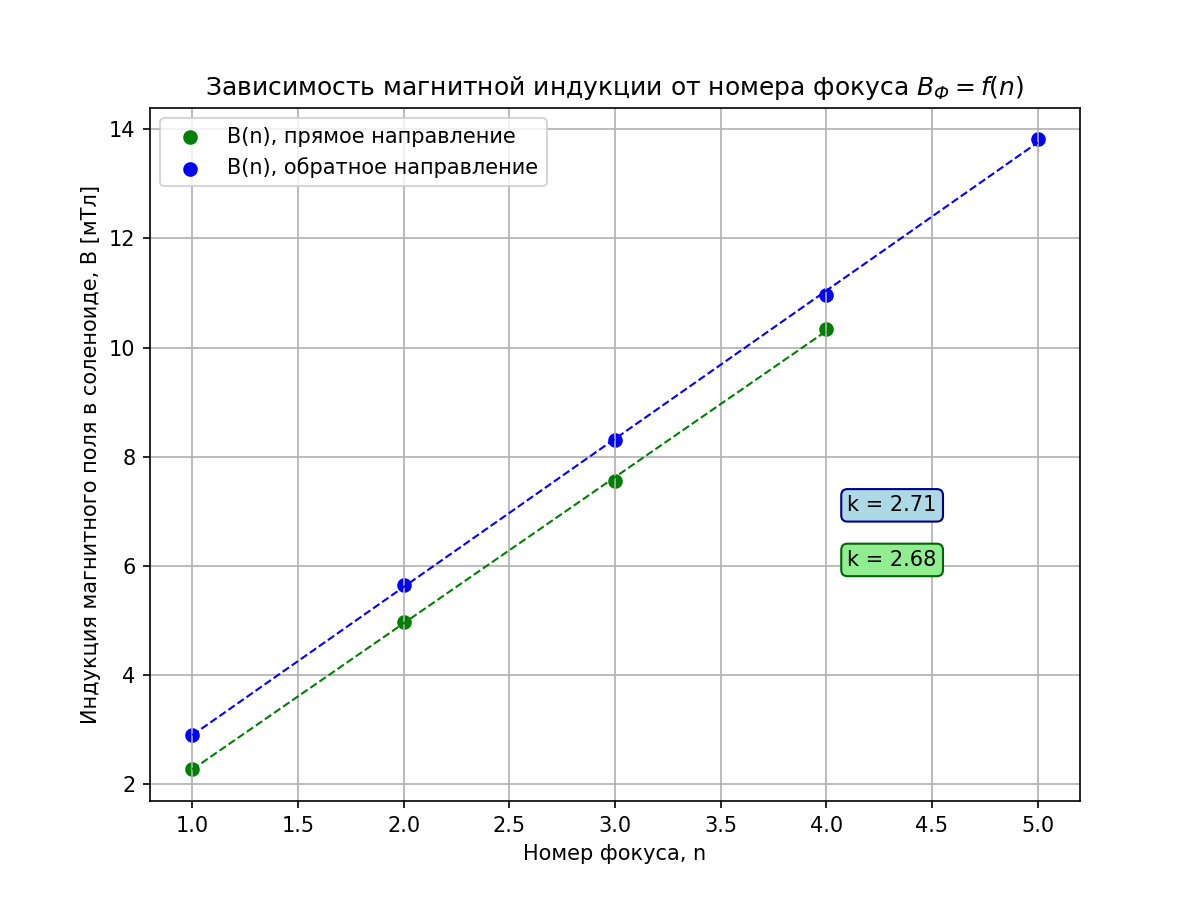
\includegraphics[width=1\textwidth]{focus.png}
    \label{fig:focus}
\end{figure}
\subsection{Выводы}
С учетом погрешностей результаты совпадают с табличными и в первом, и во втором случае. Но относительная погрешность порядка 50 процентов говорит о большом количестве случайных ошибок, допущенных при измерениях.
\newpage
\section{Метод магнетрона}
\begin{itemize}
	\item \textbf{Цель работы:} Определение отношения заряда электрона к его массе методом магнетрона.
    \item \textbf{В работе используются:} Электронная лампа с цилиндрическим анодом; универсальный стабилизированный источник постоянного и переменного напряжений; соленоид; миллиамперметр; амперметр и вольтметр постоянного тока.
\end{itemize}

\subsection{Экспериментальная установка}
\begin{figure}[H]
    \centering
    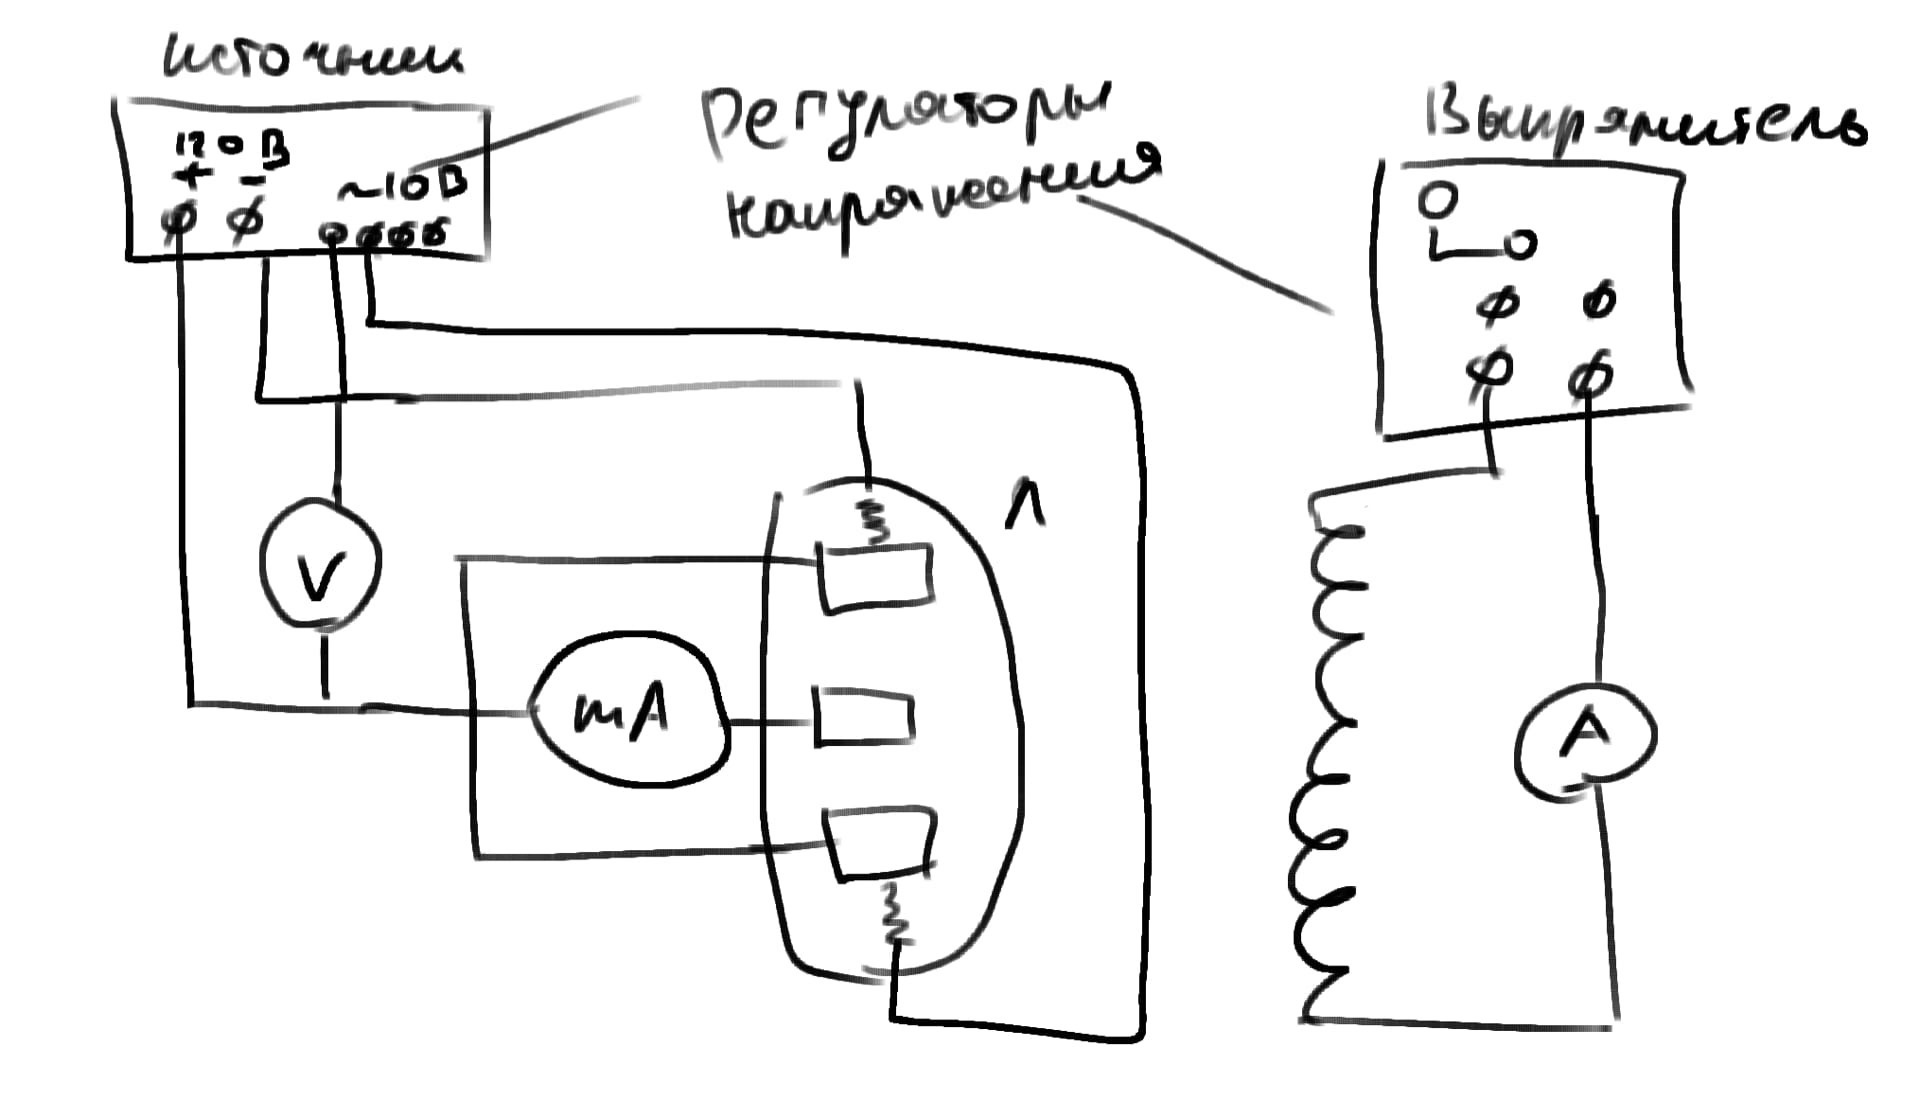
\includegraphics[width=0.7\textwidth]{set1}
    \caption{Схема установки}
    \label{fig:set1}
\end{figure}
\subsection{Теоретические сведения}
В так называемом методе магнетрона отношение $e / m$ измеряется на основе исследования движения электрона в скрещенных электрическом и магнитном полях, перпендикулярных друг другу. Название метода связано с тем, что такая конфигурация электрического и магнитного полей реализуется в магнетронах --- генераторах электромагнитных колебаний сверхвысоких частот.

Для уяснения идеи метода магнетрона, рассмотрим вначале движение заряда в <<плоском магнетроне>>б который можно представить себе в виде плоского конденсатора, помещённого в магнитное поле так, что $\boldsymbol{E} \perp \boldsymbol{B}$. При этом отрицательная пластина конденсатора играет роль катода, положительная соответственно анода.  Если бы магнитого поля не было, то все электроны, вылетевшие без начальной из катода такого плоского диода, попадали бы на анод. При наличии магнитного поля траектории электронов искривляются, вследствие чего при достаточно большом магнитном поле ни один электрон не достигнет анода.
Для заданного напряжения между катодом и анодом существует некоторое критическое значение магнитной индукции $B_\text{кр}$, при котором траектории касаются поверхности анода. Если $B < B_\text{кр}$, то все электроны достигают анода и ток через магнетрон имеет то же значение, что и без магнитного поля. Если же $B > B_\text{кр}$, то электроны не достигают анода и ток через лампу равен нулю.

Рассчитаем это критическое значение индукции магнитного поля. Уравнения движения электрона в нашем случае имеет вид
\begin{equation}
	m \frac{d v_x}{d t} = e v_y B,
\end{equation}
\begin{equation}
	m \frac{d v_y}{d t} = e E - e v_x B
\end{equation}
при начальных условиях $x(0) = y(0) = 0, v_x(0) = v_y (0) = 0$

Непосредственной подстановкой несложно убедиться в том, что решением системы дифференциальных уравнений с заданными начальными условиями является уравнение циклоиды (в параметрической форме):
\begin{equation}
	x = v t - R \sin \omega t, \quad y = R(1 - \cos \omega t)
\end{equation}
где $v = \frac{E}{B}, R = \frac{v}{\omega} = \frac{E m}{e B^2}$

Касание анода происходит при $2R = d$ ($d$ --- расстояние между анодом и катодом). Этому значению соответствует критическое поле
\begin{equation}
	B_\text{кр} = \frac{\sqrt{2V}}{d \sqrt{e / m}}
\end{equation}
Из последней формулы находим удельный заряд:
\begin{equation}
	\frac{e}{m} = \frac{2V}{d^2 B_\text{кр}^2}
\end{equation}
Эта формула позволяет вычислить $e / m$, если при заданном значении напряжения на аноде $V$ найти такое значение магнитного поля, при превышении которого ток в магнитроне отсутствует.

В настоящей работе отношение $e / m$ для электрона определяется с помощью метода, получившего название <<метод магнетрона>>. Это название связано с тем, что применяемая в работе конфигурация электрического и магнитного полей напоминает конфигурацию полей в магнетронах --- генераторах электромагнитных колебаний сверхвысоких частот.

Движение электронов в этом случае происходит в кольцевом пространстве, заключённом между катодом и анодом двухэлектродной электронной лампы. Нить накала лампы (катод) располагается вдоль оси цилиндрического анода, так что электрическое поле между катодом и анодом имеет радиальное направление. Лампа помещается внутри соленоида, создающего магнитное поле, параллельное оси лампы.

Рассмотрим траектории электронов, вылетевших из катода, более подробно. Пусть потенциал анода равен $V_a$. В отсутствие магнитного поля электрон движется прямолинейно по радиусу. При слабом поле траектории несколько искривляются, но электроны всё же попадают на анод. При некотором критическом значении индукции магнитного поля $B_\text{кр}$ траектории искривляются настолькко, что касаются анода. Наконец, при $B > B_\text{кр}$ электроны вовсе не попадают на анод и возвращаются к катоду. Величину $B_\text{кр}$ нетрудно найти по формуле, приведённой выше, заметив, что в этом случае радиальная скорость электрона $\dot r$ при $r = r_a$ (при радиусе анода) обращается в нуль:
\begin{equation}
	V_a = \frac{e B_\text{кр}^2 r_a^2}{8 m}
\end{equation}
Преобразуя это выражение, найдём 
\begin{equation}
	\frac{e}{m} = \frac{8 V_a}{B_\text{кр}^2 r_a^2}
\end{equation}
Эта формула позволяет вычислять $e / m$, если при заданном $V_a$ найдено значение магнитного поля (или, наоборот, при заданном $B$ такое значение $V_a$), при котором электроны перестают попадать на анод.
До сих пор мы рассматривали идеальный случай, когда при $B < B_\text{кр}$ все электроны без исключения попадают на анод, а при $B > B_\text{кр}$ все они возвращаются на катод, не достигнув анода. Анодный ток $I_a$ c увеличением магнитного поля изменялся бы при этом так, как это изображено на риснуке выше пунктирной линией. В реальных условиях невозможно обеспечить полную коаксиальность анода и катода, вектор индукции магнитного поля всегда несколько наклонён по отношению к катоду, магнитное поле не вполне однородно и так далее. Все эти причины приводят к сглаживанию кривой на рисунке выше и она приобретает вид сплошной линии. В хорошо собранной установке перелом функции $I_a = f(B)$ остаётся, однако, достаточно резким и с успехом может быть использован для измерения $e / m$.
\subsection{Обработка результатов}
Занесем в таблицу данные установки:
\begin{table}[H]
	\centering
	\begin{tabular}{|c|c|}
	\hline
	Величина & Значение \\ \hline
	K, \text{Т/A}     & $3,5 * 10^{-2}$   \\ \hline
	$r_a$, $\text{мм}$  & 12      \\ \hline
	\end{tabular}
	\caption{Данные установки}
	\label{tab:data1}
\end{table}
Снимем зависимость анодного тока от тока через соленоид при различных напряжениях на аноде лампы. Построим графики для каждого случая, учитывая что $B = kI_m$:
\begin{figure}[H]
    \centering
    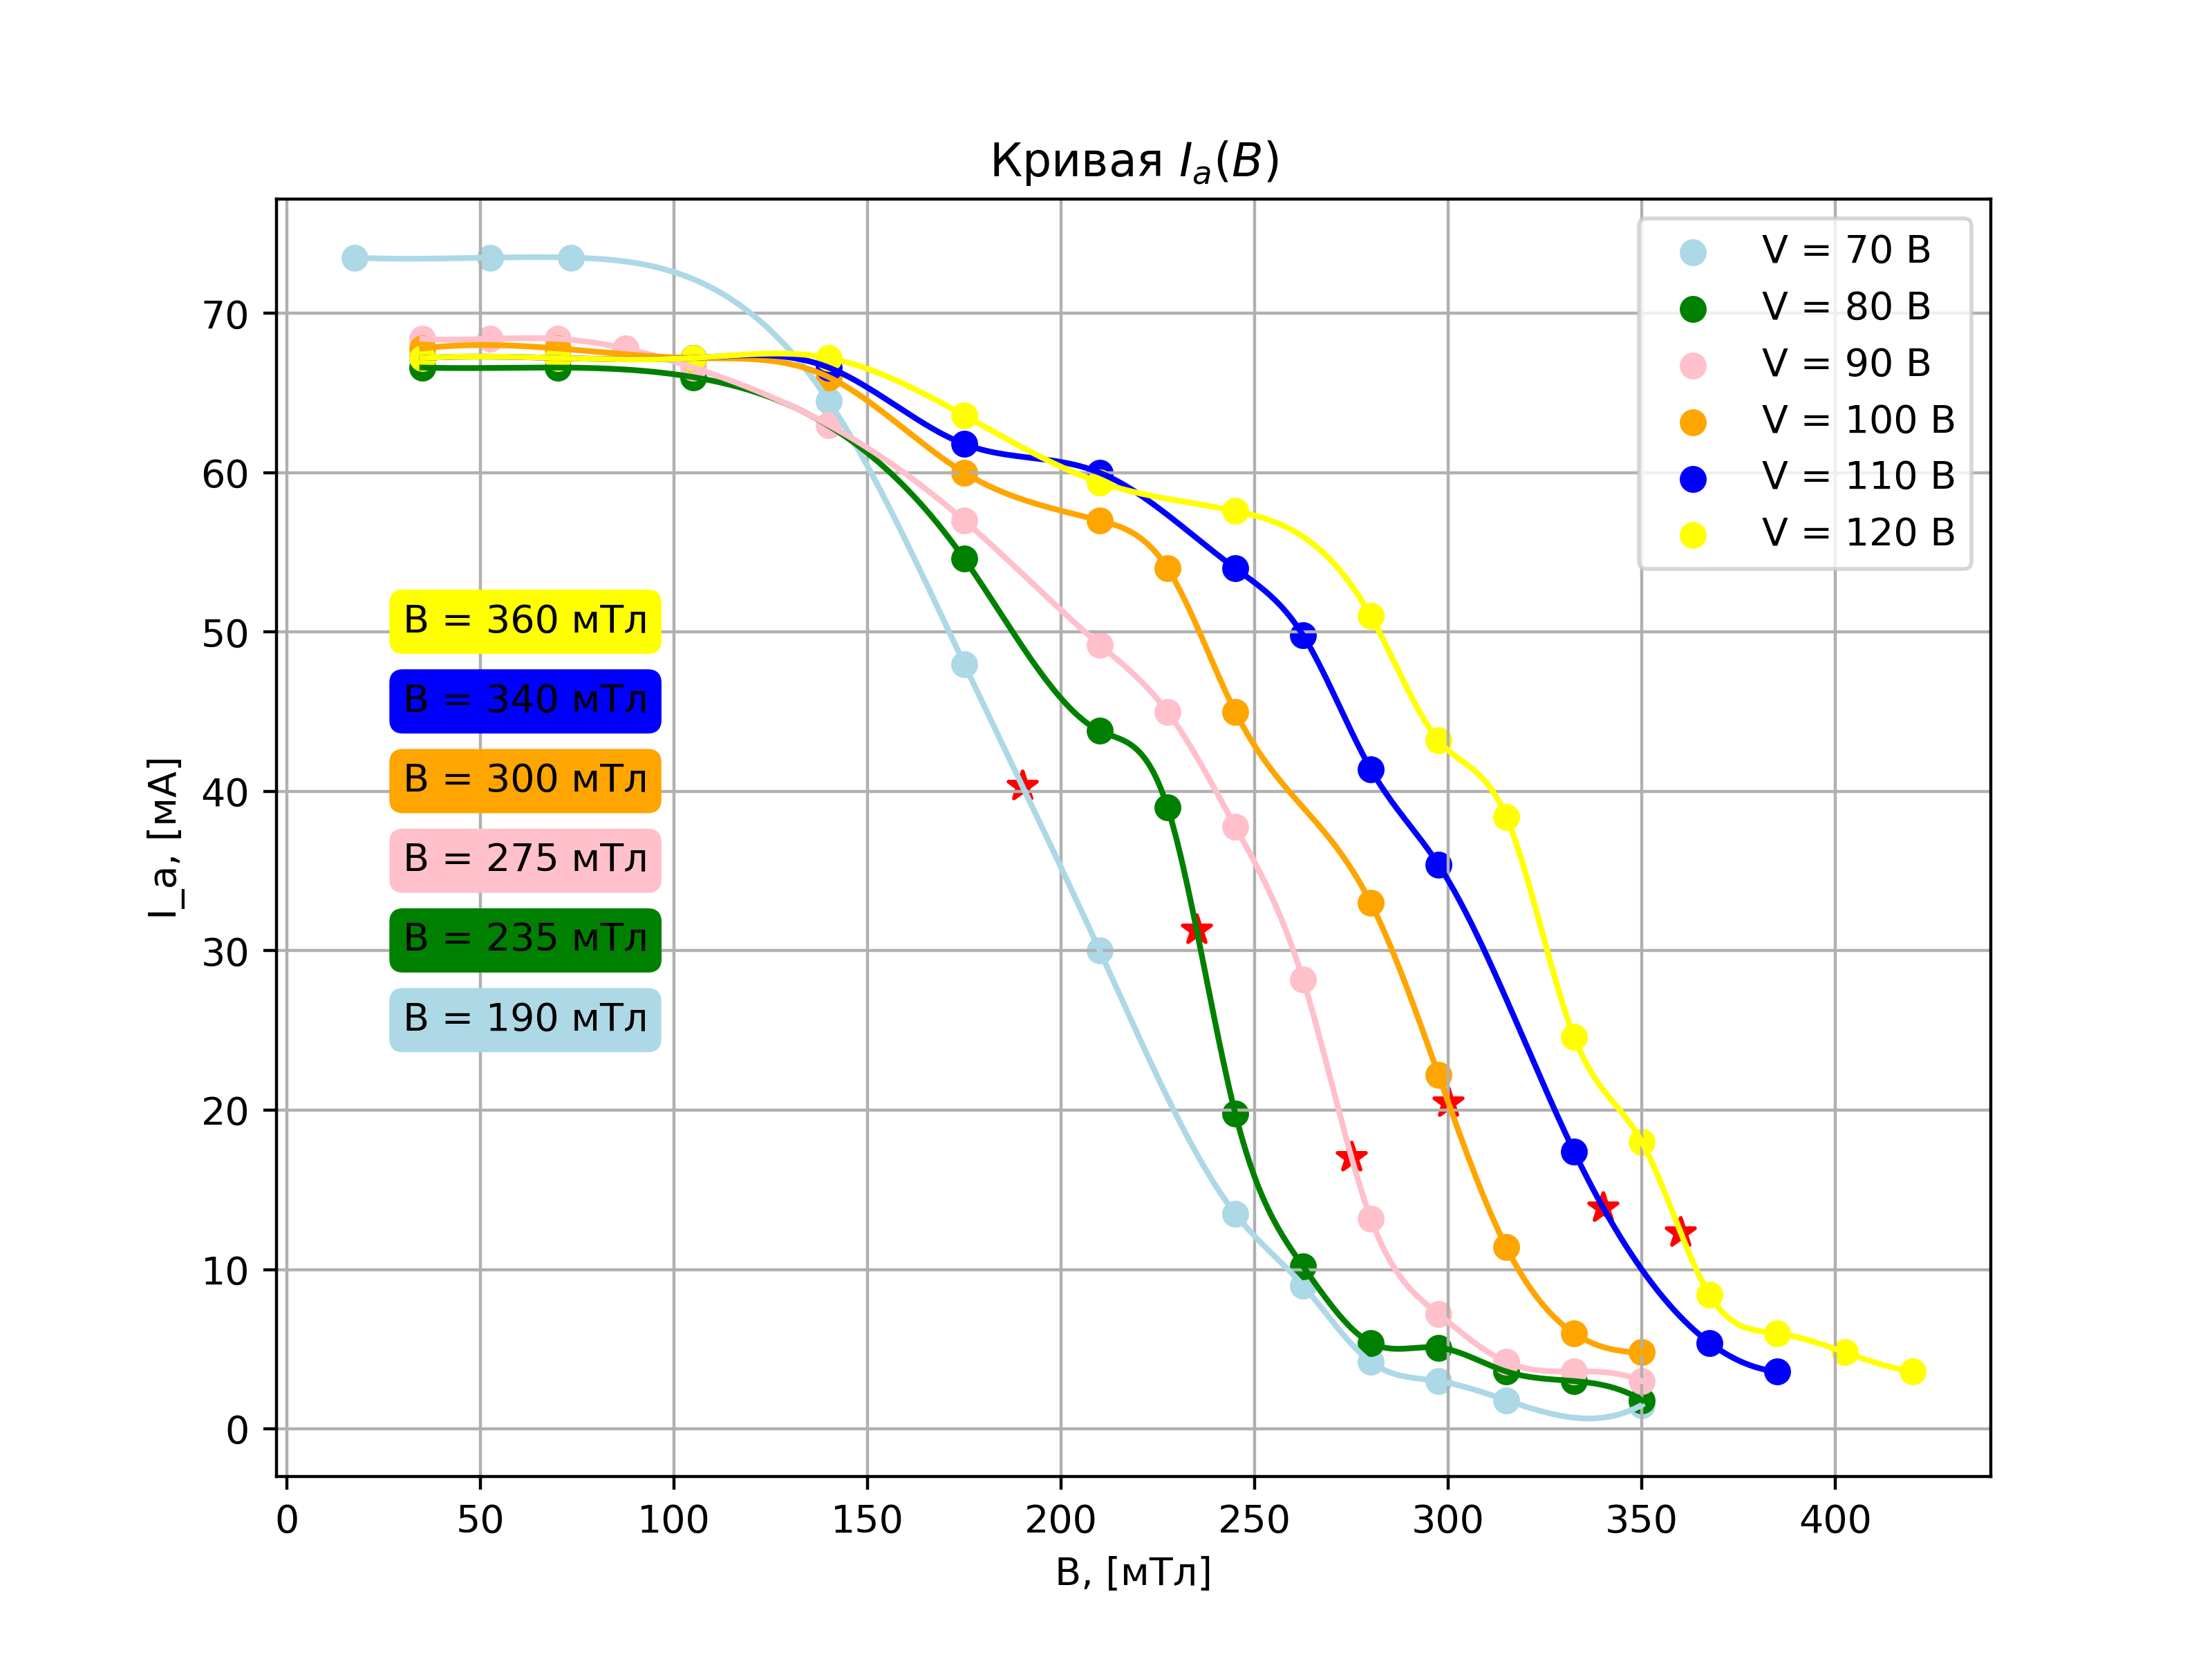
\includegraphics[width=1\textwidth]{magnetron.png}
    \label{fig:magnetron}
\end{figure}
Красным маркером на графике отмечены $B_\text{кр}$.

Построим теперь график зависимости $B^2_\text{кр}$ от напряжения на аноде лампы и найдем по полученному коэффециенту наклона прямой удельный заряд электрона:
\begin{equation}
	B^2_\text{кр} = kV \Rightarrow \frac{V}{B^2_\text{кр}} = \frac{1}{k}
\end{equation}
\begin{figure}[H]
    \centering
    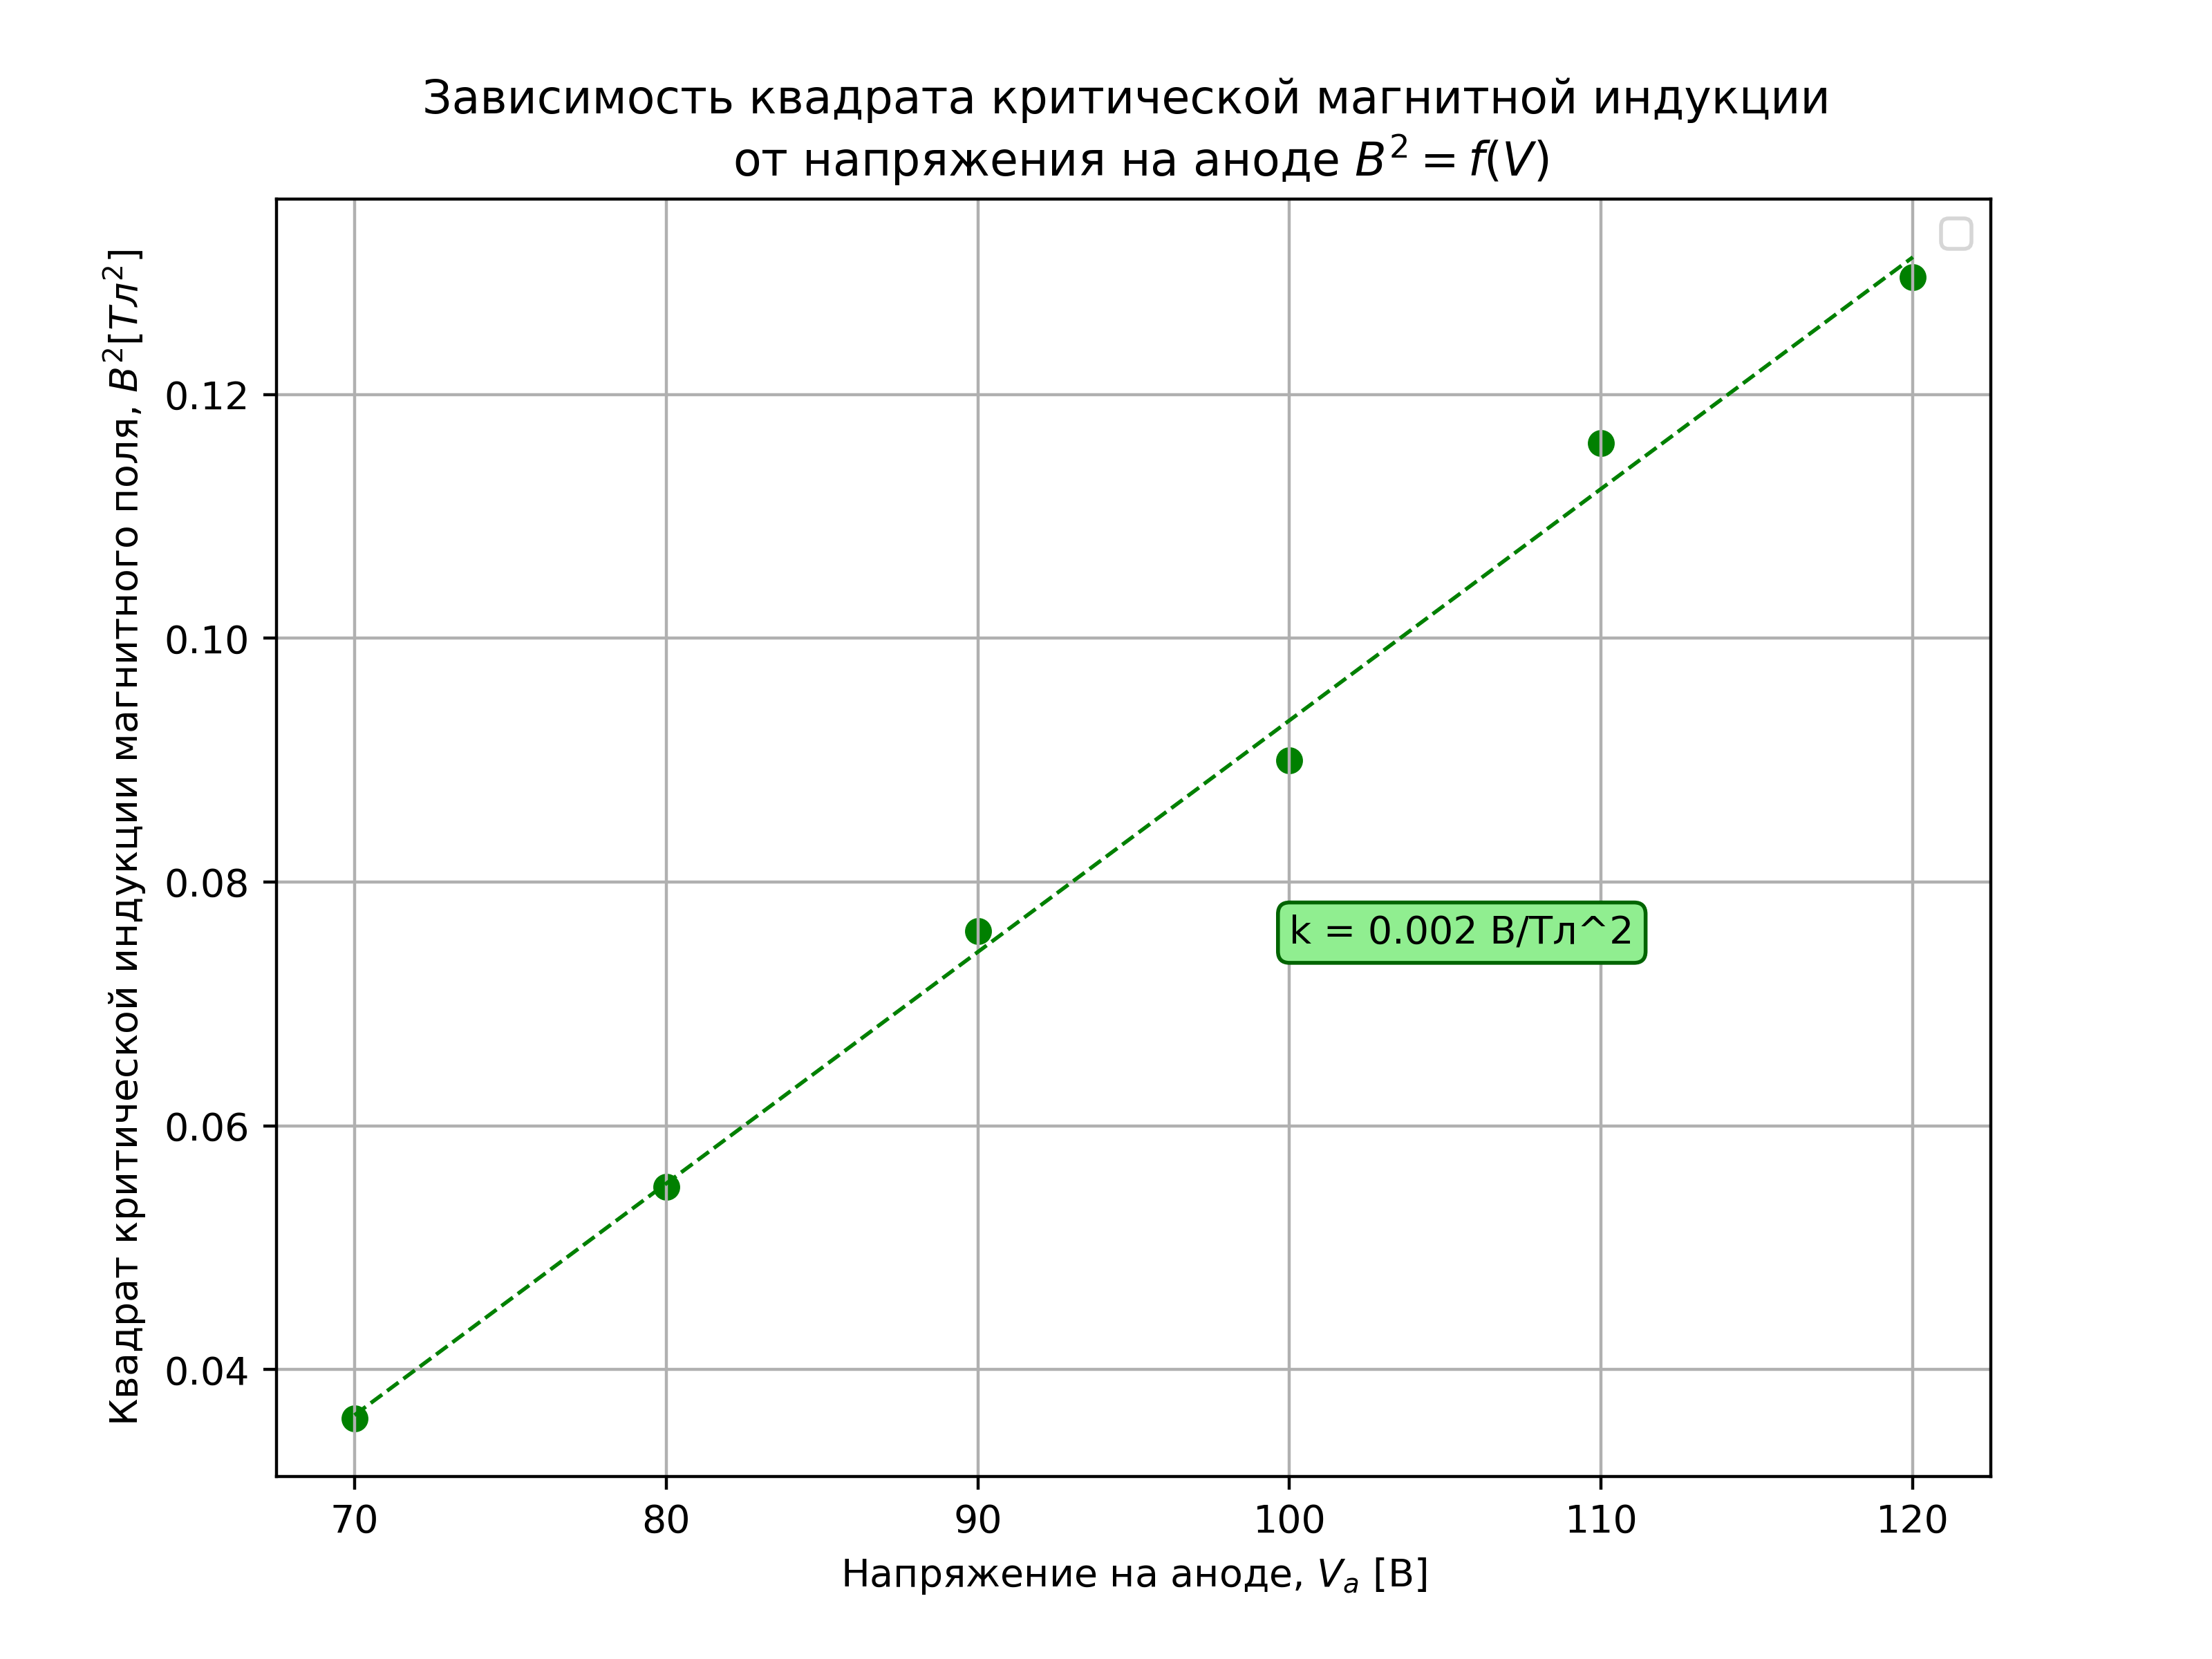
\includegraphics[width=1\textwidth]{magnetron_last.png}
    \label{fig:magnetron_last}
\end{figure}
Отсюда
\begin{equation}
	\boldmath{\frac{e}{m} = \frac{8V_a}{r^2_a B^2_\text{кр}} = (1,5 \pm 0,3) \cdot 10^{11} \text{Кл/кг}}
\end{equation}
\subsection{Выводы}
Как видно, полученное значение совпадает с табличным в пределах погрешности. Сводная таблица для обоих методов:
\begin{table}[H]
	\centering
	\begin{tabular}{|c|c|c|}
	\hline
	\textbf{Метод}        & \textbf{Удельный заряд, Кг/кл} & \textbf{Погрешность, процентов} \\ \hline
	Магнетрон             & 1,5                            & 20                     \\ \hline
	Магнитная фокусировка & 1,25                           & 48                     \\ \hline
	\end{tabular}
	\label{tab:itogi}
	\end{table}
Лучше получился метод магнетрона, так как погрешность получилась меньше.
\end{document}